\section{eo\-Combined\-Init$<$ EOT $>$ Class Template Reference}
\label{classeo_combined_init}\index{eoCombinedInit@{eoCombinedInit}}
Combined INIT: a proportional recombination of {\bf eo\-Init}{\rm (p.\,\pageref{classeo_init})} objects.  


{\tt \#include $<$eo\-Combined\-Init.h$>$}

Inheritance diagram for eo\-Combined\-Init$<$ EOT $>$::\begin{figure}[H]
\begin{center}
\leavevmode
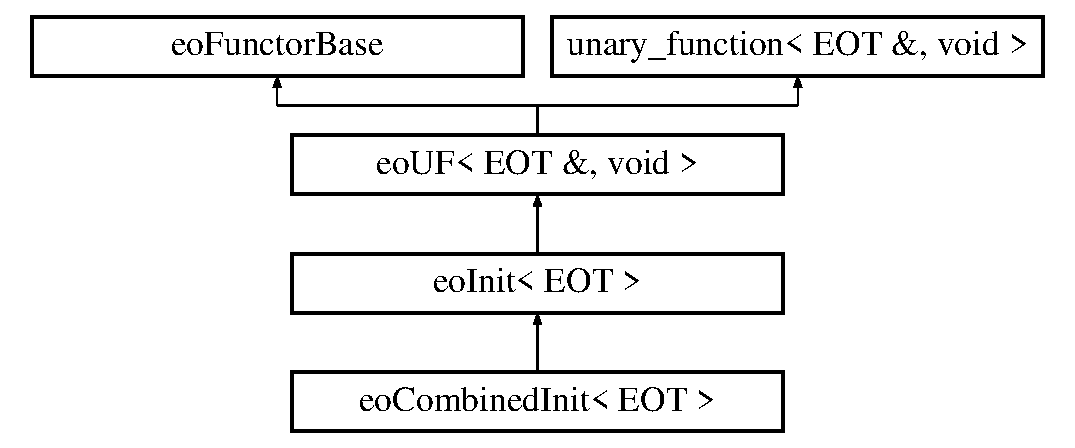
\includegraphics[height=4cm]{classeo_combined_init}
\end{center}
\end{figure}
\subsection*{Public Member Functions}
\begin{CompactItemize}
\item 
{\bf eo\-Combined\-Init} ({\bf eo\-Init}$<$ {\bf EOT} $>$ \&\_\-init, double \_\-rate)\label{classeo_combined_init_a0}

\begin{CompactList}\small\item\em Ctor, make sure that at least one {\bf eo\-Init}{\rm (p.\,\pageref{classeo_init})} is present. \item\end{CompactList}\item 
void {\bf add} ({\bf eo\-Init}$<$ {\bf EOT} $>$ \&\_\-init, double \_\-rate, bool \_\-verbose=false)\label{classeo_combined_init_a1}

\begin{CompactList}\small\item\em The usual method to add objects to the combination note the \_\-verbose parameter, that allows to print what's inside the combination with scaled rates. \item\end{CompactList}\item 
virtual void {\bf print\-On} (std::ostream \&\_\-os)\label{classeo_combined_init_a2}

\begin{CompactList}\small\item\em outputs the operators and percentages \item\end{CompactList}\item 
virtual void {\bf operator()} ({\bf EOT} \&\_\-eo)\label{classeo_combined_init_a3}

\begin{CompactList}\small\item\em Performs the init: chooses among all initializers using roulette wheel on the rates. \item\end{CompactList}\item 
virtual std::string {\bf class\-Name} (void) const 
\begin{CompactList}\small\item\em class\-Name: Mandatory because of eo\-Combined\-Init. \item\end{CompactList}\end{CompactItemize}
\subsection*{Private Attributes}
\begin{CompactItemize}
\item 
std::vector$<$ {\bf eo\-Init}$<$ {\bf EOT} $>$ $\ast$ $>$ {\bf initializers}\label{classeo_combined_init_r0}

\item 
std::vector$<$ double $>$ {\bf rates}\label{classeo_combined_init_r1}

\end{CompactItemize}


\subsection{Detailed Description}
\subsubsection*{template$<$class EOT$>$ class eo\-Combined\-Init$<$ EOT $>$}

Combined INIT: a proportional recombination of {\bf eo\-Init}{\rm (p.\,\pageref{classeo_init})} objects. 



Definition at line 35 of file eo\-Combined\-Init.h.

\subsection{Member Function Documentation}
\index{eoCombinedInit@{eo\-Combined\-Init}!className@{className}}
\index{className@{className}!eoCombinedInit@{eo\-Combined\-Init}}
\subsubsection{\setlength{\rightskip}{0pt plus 5cm}template$<$class EOT$>$ virtual std::string {\bf eo\-Combined\-Init}$<$ {\bf EOT} $>$::class\-Name (void) const\hspace{0.3cm}{\tt  [inline, virtual]}}\label{classeo_combined_init_a4}


class\-Name: Mandatory because of eo\-Combined\-Init. 

SHould be pure virtual, but then we should go over the whole code to write the method for all derived classes ... MS 16/7/04 

Reimplemented from {\bf eo\-Init$<$ EOT $>$} {\rm (p.\,\pageref{classeo_init_a0})}.

Definition at line 81 of file eo\-Combined\-Init.h.

Referenced by eo\-Combined\-Init$<$ EOT $>$::print\-On().

The documentation for this class was generated from the following file:\begin{CompactItemize}
\item 
eo\-Combined\-Init.h\end{CompactItemize}
